\documentclass[xcolor=table]{beamer}
% Class options include: notes, notesonly, handout, trans, hidesubsections, shadesubsections, inrow, blue, red, grey, brown
% beamer loads automatically: xcolor, amsmath, amsthm, calc, geometry, hyperref, extsizes

%%%%%%%%%%%%% Packages %%%%%%%%%%%%%
\usepackage{beamerthemesplit}
\usepackage[ngerman,english]{babel}
%\usepackage{lmodern} % verbessert verwendete Schriftart
%\usepackage{times}
\usepackage{amsmath}
\usepackage{listings}
\usepackage{calc}
\usepackage[labelfont={color=DBbluedark,bf}, font={color=DBbluedark,footnotesize}]{caption}
\usepackage{geometry}
\usepackage{fontspec}
\usepackage{enumitem}
\usepackage{multicol}
\usepackage[draft]{pdfcomment}


%%%%%%%%%%%%% Settings %%%%%%%%%%%%%
\beamertemplatenavigationsymbolsempty% suppress the navigation bar
\setbeamertemplate{caption}[numbered] % Caption haben eine Nummer

%\beamertemplategridbackground[\abstand] % hinterlegt ein Gitter

\rowcolors{2}{lightgray!20}{lightgray!40} % alternierende Zeilenfarbe
\renewcommand{\arraystretch}{1.2}

\newcommand{\comment}[1]{}


%%%%%%%%%%%%%% Layout
\newcommand{\abstand}{\dimexpr\paperwidth/21\relax}
\setbeamersize{text margin left=\abstand,text margin right=\abstand}
\setlength{\columnsep}{\abstand}
\setlength{\unitlength}{1in}% beamer: 5" x 3.75" (4:3)

%%%%%%%%%%%%%% Fonts 
\setmainfont{Arial}
\setsansfont{Arial}
\setmonofont{Fira Mono}%Fira Mono, Ricty Diminished Discord
\renewcommand\UrlFont{\rmfamily} % passt URL an


%%%%%%%%%%%%%% Titlepage
\setbeamerfont{title}{size=\LARGE}
\setbeamerfont{subtitle}{size=\Large}
\setbeamerfont{author}{size=\small}
\setbeamerfont{date}{size=\small}
\setbeamerfont{institute}{size=\scriptsize}

\defbeamertemplate*{title page}{customized}[1][]
{\centering\vspace{\baselineskip}
    \color{FUblue}\usebeamerfont{title}\inserttitle\par
    \usebeamerfont{subtitle}%
    \vspace{0.5\baselineskip}
    \usebeamercolor[fg]{subtitle}\insertsubtitle\par
    \vspace{1\baselineskip}
    \usebeamerfont{author}\insertauthor\par
    \vspace{1.5\baselineskip}
    \textcolor{DBblue}{\rule{\textwidth}{1pt}}\par
    \vspace{2\baselineskip}
    \usebeamerfont{institute}\insertinstitute\par
    \vspace{1.5\baselineskip}
    \small\usebeamerfont{date}\insertdate\par
  %\usebeamercolor[fg]{titlegraphic}\inserttitlegraphic
}

% \insertshortinstitute
% \insertshorttitle
% \insertshortauthor
% \insertshortdate
% \insertframenumber
% \inserttotalframenumber
% \thesection
% \insertsection

%%%%%%%%%%%%%% Headline 
\setbeamertemplate{headline}{%
%   \leavevmode% horizontal mode is entered
%   \begin{beamercolorbox}[wd=\paperwidth,
% 	ht=2ex, dp=1ex, leftskip=1pt,left]%
%     {section in head/foot}
%     \insertsectionnavigationhorizontal{\paperwidth}{}{\hskip0pt plus1filll}
%   \end{beamercolorbox}%
%   \vskip0pt
%   \begin{beamercolorbox}[wd=\paperwidth,
%     ht=4ex, dp=1.125ex]%
%     {subsection in head/foot}
%     \insertsubsectionnavigationhorizontal%
%       {\paperwidth}{}{\hskip0pt plus1filll}
%   \end{beamercolorbox}
}


%%%%%%%%%%%%%% frametitle
\setbeamerfont{frametitle}{size=\large}
\setbeamertemplate{frametitle}{%
  \vskip-2pt
  \begin{beamercolorbox}[wd=\paperwidth, ht=2.5ex, dp=1.25ex, left]{frametitle}%
    \hskip\abstand%
    \insertframetitle
  \end{beamercolorbox}%
  \vskip-1pt%
  \begin{beamercolorbox}[wd=\paperwidth,
    ht=1.2ex, dp=0.55ex, left]%
    {subsection in head/foot}%
    \tiny%
    \insertsectionnavigationhorizontal%
      {\paperwidth}{\hskip\dimexpr0.5\abstand\relax}%
      {\hskip0pt plus1filll}% glue stretching
  \end{beamercolorbox}
}

%%%%%%%%%%%%%% Footline 
\newcommand{\footlinetext}{
\insertshortauthor\vskip1.5pt
\insertshortdate}

\setbeamerfont{footline}{size=\tiny,
series=\normalfont}

\setbeamertemplate{footline}{
% erzeugt den Fortschrittsbalken
\color{DBblue!60}%!60
\rule{\dimexpr\textwidth*\insertframenumber/\inserttotalframenumber\relax}{2pt}% horizontal line
\color{FUgreen!60}%
\rule{\dimexpr\textwidth-\textwidth*\insertframenumber/\inserttotalframenumber\relax}{2pt}
\vskip0pt%
% fügt Daten hinzu
\leavevmode% horizontal mode is entered
\hspace{\abstand}%
\begin{beamercolorbox}% Logo
  [wd=\abstand, ht=\dimexpr\abstand+1.5pt\relax, dp=1.5pt, left]
  {whitebox}%
  
\includegraphics[height=\abstand]{img/agdb-logo}
\end{beamercolorbox}%
\hspace{0.5\abstand}%
\begin{beamercolorbox}% Titel
  [wd={\dimexpr\paperwidth-10\abstand\relax},
  ht=\dimexpr\abstand+1.5pt\relax, dp=1.5pt, left]% leftskip=2ex
  {whitebox}%
  \raisebox{6.75pt}{%
  \begin{minipage}{\linewidth}
  \footlinetext
  \end{minipage}}
\end{beamercolorbox}%
\hfill%
\begin{beamercolorbox}% Logo
  [wd=5\abstand, ht=\dimexpr\abstand+1.5pt\relax, dp=1.5pt, right]
  {whitebox}%
  
\includegraphics[height=\abstand]
  {img/FULogo_RGB}\hspace{0.5\abstand}
\end{beamercolorbox}%
\ifnum\value{framenumber}<1%
  \begin{beamercolorbox}% Seitennummer
    [wd=\abstand, ht=\dimexpr\abstand+1.5pt\relax,
    dp=1.5pt, center]
    {whitebox}%
  \end{beamercolorbox}%
\else%
  \begin{beamercolorbox}% Seitennummer
    [wd=\abstand, ht=\dimexpr\abstand+1.5pt\relax,
    dp=1.5pt, center]
    {framenumber}%
    \raisebox{2.2ex}{\textnormal{%
    \insertframenumber{}%~/~\inserttotalframenumber
    }}
  \end{beamercolorbox}%
\fi%
}


%%%%%%%%%%%%%% TOC 
\setbeamertemplate{section in toc}[sections numbered]
\setbeamertemplate{subsection in toc}[subsections numbered]
\setbeamertemplate{section in toc}{ \textbf{\textcolor{DBblue}{\inserttocsectionnumber}}~\inserttocsection\par}
\setbeamertemplate{subsection in toc}{\hspace{0.6em}\color{FUblue!80}\inserttocsectionnumber.\inserttocsubsectionnumber~\inserttocsubsection\par}

\setcounter{tocdepth}{1} % TOC enthält section bis subsection


%%%%%%%%%%%%%% Enumitem 
\setlist[enumerate]{font=\color{DBblue}\bfseries, leftmargin=*}
\setlist[enumerate,1]{label=\arabic*, ref=\arabic*}
\setlist[enumerate,2]{label*=.\arabic*, ref=\theenumi.\arabic*}
\setlist[enumerate,3]{label*=.\arabic*, ref=\theenumii.\arabic*}
\setlist[itemize]{font=\color{DBblue}\bfseries, leftmargin=*}
\setlist[itemize,1]{label=%
	$\blacktriangleright$, ref=\labelitemi}
\setlist[itemize,2]{label=\small%
	$\blacktriangleright$, ref=\labelitemii} % \bullet
\setlist[itemize,3]{label=\footnotesize%
	$\blacktriangleright$, 
    ref=\labelitemiii}%textbullet, diamond
\setlist[description]{font=\color{DBblue}\bfseries, leftmargin=*}


%%%%%%%%%% Referenzen %%%%%%%%%%%
\usepackage[style=numeric, bibencoding=utf8, backend=biber, sorting=none, maxbibnames=99]{biblatex}% für bibliographie, style=authortitle/numeric/ieee, backend=biber/bibtex/bibtex8, bibencoding=ascii/utf8
\setbeamertemplate{bibliography item}{\insertbiblabel} % setzt Nummerierung im Lit.Verzeichnis
\usepackage{csquotes} % notwendig, wenn man babel und bibtex benutzt
\usepackage{silence}% Filter warnings issued by package biblatex starting with "Patching footnotes failed"
\WarningFilter{biblatex}{Patching footnotes failed}
\addbibresource{src/bibliography.bib}
% redefines Styles
\DeclareFieldFormat{isbn}{}

\usepackage{xpatch}
\xpatchbibmacro{author}{\printnames{author}}{\mkbibbold{\printnames{author}}}{}{} % author bold


%%%%%%%%%%%%% Farben %%%%%%%%%%%%%
\let\definecolor=\xdefinecolor
\definecolor{FUgreen}{RGB}{153,204,0}
\definecolor{FUblue}{RGB}{0,51,102}
\definecolor{DBblue}{RGB}{0,102,204}
\definecolor{DBbluedark}{RGB}{0,51,102}

\setbeamercolor{palette primary}{bg=FUblue,fg=white}
\setbeamercolor{palette secondary}{bg=FUblue,fg=white}
\setbeamercolor{palette tertiary}{bg=FUblue,fg=white}
\setbeamercolor{palette quaternary}{bg=FUblue,fg=white}
\setbeamercolor{title}{fg=DBbluedark, bg=white}
\setbeamercolor{subtitle}{fg=DBbluedark, bg=white}
\setbeamercolor{titlelike}{parent=structure}
\setbeamercolor{author}{fg=DBbluedark, bg=white}
\setbeamercolor{frametitle}{fg=white,bg=FUblue}
\setbeamercolor{section in head/foot}{fg=DBbluedark,bg=white}
\setbeamertemplate{section in head/foot shaded}[default][50]
\setbeamercolor{subsection in head/foot}{fg=DBbluedark,bg=lightgray}
\setbeamercolor{framenumber}{fg=white, bg=FUblue}
\setbeamercolor{whitebox}{fg=DBbluedark,bg=white}
% Standard block
\setbeamercolor{block title}{fg=white, bg=FUblue}
\setbeamercolor{block body}{fg=DBbluedark, bg=lightgray!30}
% Alert block
\setbeamercolor{block title alerted}{fg=white, bg=red}
\setbeamercolor{block body alerted}{fg=DBbluedark, bg=red!20}
% Example block
\setbeamercolor{block title example}{fg=white, bg=FUblue}
\setbeamercolor{block body example}{fg=DBbluedark, bg=lightgray!30}
\setbeamercolor{itemize item}{fg=DBblue} % all frames will have red bullets
\setbeamercolor{enumerate item}{fg=DBblue}

\hypersetup{
    colorlinks,
    linktocpage,
    allcolors=FUblue,
    urlcolor=DBblue,
    %linkcolor=red, % färbt auch Menü und Shorttitle
    breaklinks
}
% setzt die globale Schriftfarbe auf DBbluedark
\makeatletter
\newcommand{\globalcolor}[1]{%
  \color{#1}\global\let\default@color\current@color
}
\makeatother
\AtBeginDocument{\globalcolor{DBbluedark}}

% Bibliography entries:
\setbeamercolor{bibliography entry author}{fg=FUblue}
\setbeamercolor{bibliography entry title}{fg=FUblue} 
\setbeamercolor{bibliography entry location}{fg=FUblue} 
\setbeamercolor{bibliography entry note}{fg=FUblue}
\setbeamercolor{bibliography item}{fg=DBblue}

%%%%%%%%%%%% Blocks %%%%%%%%%%%%%
% passt die Größe der Blöcke an \linewidth an an zieht den Rand ab, den die Blöcke mit sich bringen
\addtobeamertemplate{block begin}{\flushright\setlength{\textwidth}{\linewidth-0.5\abstand}}{}
\addtobeamertemplate{block example begin}{\flushright\setlength{\textwidth}{\linewidth-0.5\abstand}}{}
\addtobeamertemplate{block alerted begin}{\flushright\setlength{\textwidth}{\linewidth-0.5\abstand}}{}

%%%%%%%%%%%% Umgebung %%%%%%%%%%%%
\newenvironment{frameWithPicture}[2]{% BEGIN
  \begingroup%
  \setbeamertemplate{background}{%
    \begin{picture}(5,3.75)(0,-0.27)
      \includegraphics[width = \paperwidth,
      height=\dimexpr\paperheight-5.5ex-6pt-\abstand\relax,
      %keepaspectratio
      ]{#2}
    \end{picture}%
  }%
  \begin{frame}{#1}
}
{% END
  \end{frame}%
  \endgroup%
}

%%%%%%%%%%%%%%%%%% Listings %%%%%%%%%%%%%%%%%%%
\renewcommand{\lstlistingname}{Source Code}% Listing -> Source Code
\lstloadlanguages{Python, R, HTML, Haskell, Java, SQL} 
\lstset{
   basicstyle=\color{DBbluedark}\small\ttfamily\selectfont,	% \scriptsize the size of the fonts that are used for the code
   backgroundcolor = \color{gray!20},	% legt Farbe der Box fest
   breakatwhitespace=false,	% sets if automatic breaks should only happen at whitespace
   breaklines=true,			% sets automatic line breaking
   captionpos=b,				% sets the caption-position to bottom, t for top
   commentstyle=\color{gray}\selectfont,% comment style
   frame=single,				% adds a frame around the code
   keepspaces=true,			% keeps spaces in text, useful for keeping indentation
							% of code (possibly needs columns=flexible)
   keywordstyle=\bfseries\color{DBblue}\selectfont,% keyword style
   ndkeywordstyle=\color{DBbluedark}\bfseries\selectfont,
   numbers=left,				% where to put the line-numbers;
   							% possible values are (none, left, right)
   numberstyle=\scriptsize\color{FUblue}\selectfont,	% the style that is used for the line-numbers
   numbersep=9pt,			% how far the line-numbers are from the code
   stepnumber=1,				% nummeriert nur jede i-te Zeile
   showspaces=false,			% show spaces everywhere adding particular underscores;
							% it overrides 'showstringspaces'
   %showstringspaces=false,	% underline spaces within strings only
   showtabs=false,			% show tabs within strings adding particular underscores
   flexiblecolumns=false,
   %tabsize=1,				% the step between two line-numbers. If 1: each line will be numbered
   stringstyle=\color{red}\ttfamily\selectfont,	% string literal style
   numberblanklines=false,				% leere Zeilen werden nicht mitnummeriert
   xleftmargin=\dimexpr\abstand+2pt\relax,	% Abstand zum linken Layoutrand
   framexleftmargin=\dimexpr\abstand-2pt\relax,
   xrightmargin=\dimexpr\abstand+2pt\relax,					% Abstand zum rechten Layoutrand
   framexrightmargin=\dimexpr\abstand-2pt\relax,
   aboveskip=2ex, 
}

\lstdefinestyle{html}{
   language=HTML,
}
\lstdefinestyle{hs}{
   language=Haskell,
}
\lstdefinestyle{sql}{
   language=SQL,
}
\lstdefinestyle{pseudo}{
   language = Python,
   mathescape = true,
   keywords = {do, procedure, end, while, if, else},
}
\lstdefinestyle{java}{
	language=Java,
    keywords={typeof, new, true, false, catch, function, return, null, catch, switch, var, if, in, while, do, else, case, break},
    ndkeywords={class, export, boolean, throw, implements, import, this},
	extendedchars=true,% lets you use non-ASCII characters;
    % for 8-bits encodings only, does not work with UTF-8
}
\lstdefinestyle{R}{
	language=R,
	extendedchars=true,% for 8-bits encodings only,
    % does not work with UTF-8
}


%%%%%%%%%%%%% Title, Author %%%%%%%%%%%%%
\subtitle[Short Title]{Development, Implementation and Evaluation of a Security Concept for the Secure Transfer of Sensitive Personal Data Between Different Devices}
%\title[Title]{Development, Implementation and Evaluation of a Security Concept for the Secure Transfer of Sensitive Personal Data Between Different Devices}
%\title[Development, Implementation and Evaluation of a Security Concept for the Secure Transfer of Sensitive Personal Data Between Different Devices]{Development, Implementation and Evaluation of a Security Concept for the Secure Transfer of Sensitive Personal Data Between Different Devices}
\author[Oliver Junk: Security Concept for the Secure Transfer of Sensitive Personal Data]{\texorpdfstring{%
	Oliver Junk \\(4568642)}{%
    Oliver Junk (4568642)}%
}
\institute[Institute of Computer Science]{Freie Universität Berlin, Department of Mathematics and Computer Science,\\Institute of Computer Science, Databases and Information Systems Group}
%\subject{Subject}
\date[January 15, 2020]{January 15, 2020}


\begin{document}
%%%%%%%%%%%%% Titlepage %%%%%%%%%%%%%
\begin{frame}[noframenumbering]% plain
  \titlepage
\end{frame}

%%%%%%%%%%%%% TOC %%%%%%%%%%%%%
\begin{frame}[noframenumbering]{Outline}% plain
  \tableofcontents
\end{frame}

%%%%%%%%%%%%% Content %%%%%%%%%%%%%
%Introduction
\section{Motivation}

%
\begin{frame}{Motivation}
\begin{itemize}
    \item With advances in information technology more personal data is gathered, stored and shared
    \item Disclosed sensitive personal data endangers an individuals right to self-determination
    \item Regulations, such as the General Data Protection Regulation (GDPR), implement law to protect an individuals right to privacy
\end{itemize}
\end{frame}

\comment{
\begin{frame}{Example}
\textit{Mr. Ronnie Coleman is taking part in a clinical trial. For this he regularly shoots photos of his skin with a special camera after applying the skin cream to be tested. In these photos a skin disease of Mr. Coleman is visible, which he wants to keep private.
One day, Mr. Coleman sends the photos from an unsecured network. The data is intercepted by a malicious hacker. The hacker blackmails Mr. Coleman with the publication of the photos. Mr. Coleman agrees to the demands of the blackmailer for fear of losing his job or being socially marginalized.}
\end{frame}
}

\begin{frame}{Outline of Contribution}
\begin{itemize}
    \item Design of a security concept for the transfer of sensitive personal data complying with the GDPR
    \item Design of the concept as part of the CliniScale project
    \item Evaluation of the security level of the concept by performing a security risk assessment
    \item Creation of a guideline for the implementation of identified security measurements
\end{itemize}
\end{frame}


\section{Background}
\comment{
\begin{frame}{Definitions [1/2]}
\begin{itemize}[label={}]
    \item The \textbf{General Data Protection Regulation (GDPR)} is a regulation in European Union (EU) law on data protection and privacy for all individuals within the EU and the European Economic Area implemented on May 25, 2018 \cite{GDPR}
    \item
    \item Personal data which are by their nature particularly sensitive in relation to fundamental rights and freedoms, are defined as \textbf{Sensitive Personal Data}
\end{itemize}
\end{frame}
}

\begin{frame}{Tools}
\begin{itemize}[label={}]
    \item The \textbf{Microsoft Threat Modeling Tool (MTMT)} is a core element of the Microsoft Security Development Lifecycle. It allows software architects to identify and mitigate security issues early in the process of designing a software architecture.
    \item
    \item Microsoft \textbf{STRIDE} is a threat model that supports security analysts in identifying possible threats in six different categories.
    \item
    \item The \textbf{Yakindu Security Analyst} is a tool created by the Itemis AG to perform risk assessments.
\end{itemize}
\end{frame}


\begin{frame}{Related Work [1/2]}
\begin{itemize}
    \item \textbf{J. Eichler and D. Angermeier.} “Modular Risk Assessment for the Development of Secure Automotive Systems”. In: \textit{31. VDI/VW-Gemeinschaftstagung Automotive Security}, 2015 \cite{mora}
    \item \textbf{J. Eichler, D. Angermeier, and A. Nieding.} “Systematic Identification of Security Goals and Threats in Risk Assessment”. In: \textit{Softwaretechnik-Trends 36.3}, 2016 \cite{morasecgoals}
    \item \textbf{J. Eichler, D. Angermeier, and A. Nieding.} "Supporting Risk Assessment with the Systematic Identification, Merging and Validation of Security Goals". In: \textit{Risk Assessment and Risk-Driven Quality Assurance. RISK 2016}, 2017, pp. 82–95 \cite{angermeier2016systematic}
\end{itemize}
\end{frame}

\begin{frame}{Related Work [2/2]}
\begin{itemize}
    \item \textbf{M. de Gramatica, K. Labunets, F. Massacci, F. Paci, and A. Tedeschi.} “The role of catalogues of threats and security controls in security risk assessment: an empirical study with ATM professionals”. In: \textit{International Working Conference on Requirements Engineering: Foundation for Software Quality.} Springer. 2015, pp. 98–114 \cite{cataloguerole}
    \item \textbf{W. Wilkowska and M. Ziefle.} “Privacy and data security in E-health: Requirements from the user’s perspective”. In: \textit{Health Informatics Journal 18.3}, 2012, pp. 191–201 \cite{wilkowska2012privacy}
    \comment{
    \item \textbf{E. Chin, A. P. Felt, V. Sekar, and D. Wagner.} “Measuring user confidence in smartphone security and privacy”. In: \textit{Proceedings of the eighth symposium on usable privacy and security}. ACM. 2012, p. 1 \cite{chin2012measuring}
    }
\end{itemize}
\end{frame}


\section{Analysis}
\begin{frame}{General Data Protection Regulation [1/3]}
 \begin{figure}[H]
  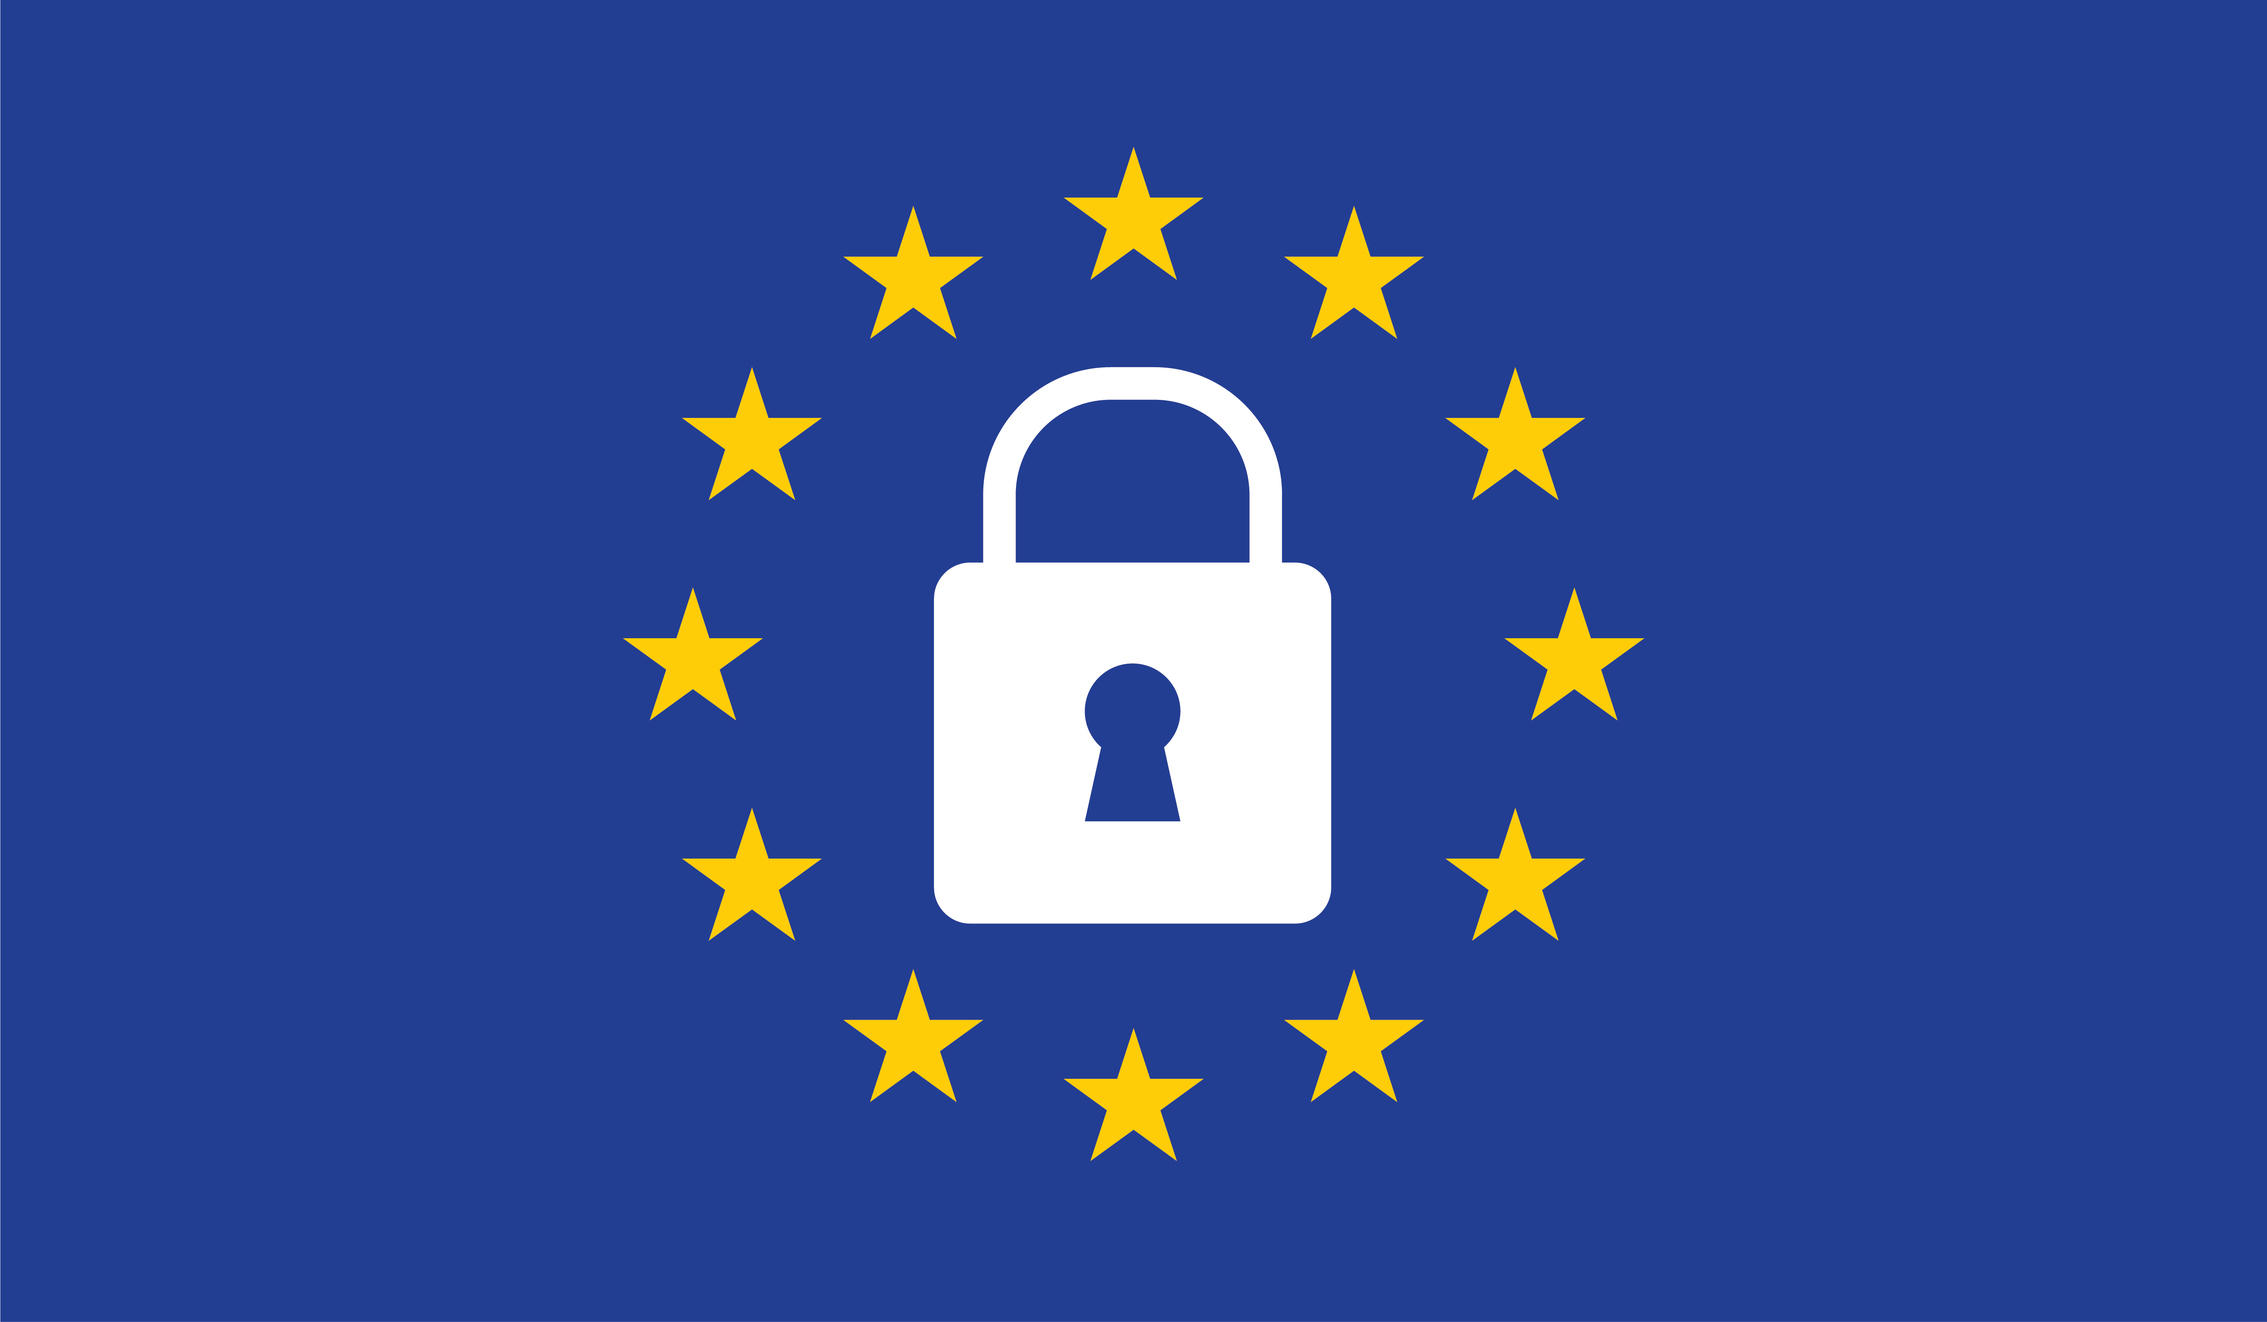
\includegraphics[width=0.3\linewidth]{img/gdpr.jpg}
  \label{fig:gdpr}
  \captionsetup{labelformat=empty}
  \caption{https://www.zdnet.com/article/gdpr-an-executive-guide-to-what-you-need-to-know/}
\end{figure}
\begin{itemize}
    \item Consists of 99 articles, 173 recitals and 14 key issues \cite{GDPR}
    \item Investigated for regulatory specifications concerning a system collecting and processing sensitive personal data
\end{itemize}
\begin{itemize}[label={}]
    \item
    \item{\textbf{Article 4: Personal Data}}  Defines personal data as any information relating to an identified or identifiable natural person \cite{GDPR4}
    \item{\textbf{Article 9: Sensitive Personal Data}}  Special category of personal data \cite{GDPR9}
\end{itemize}
\end{frame}

\begin{frame}{General Data Protection Regulation [2/3]}
\begin{itemize}[label={}]
    \item{\textbf{Article 6: Lawfulness of Processing}}  Defines conditions under which the processing of personal data is lawful \cite{GDPR6}
    \item{\textbf{Article 7: Conditions for Consent}}  Defines that consent by the data subject to processing has to be given by a clear affirmative act that is freely given, specific, informed and unambiguous \cite{GDPR7}
    \item{\textbf{Article 25: Security of Processing}}  Places the responsibility to implement appropriate technical and organizational measures to secure personal data on the controller \cite{GDPR25}
    %\item{\textbf{Article 32: Data Protection by Design and by Default}}  Defines principles the controller has to implement in the process of securing personal data \cite{GDPR32}
\end{itemize}
\end{frame}

\begin{frame}{General Data Protection Regulation [3/3]}
\begin{itemize}
    \item Personal and sensitive personal data has to be secured in a manner appropriate for the risks
    \item State of the art security measurements
    \item Consent given by a clear affirmative act that is freely given, specific, informed and unambiguous
    %\item Data Protection by Design and by Default
\end{itemize}
\end{frame}

\comment{
\begin{frame}{BSI Technical Guidelines}
\begin{itemize}
    \item Technical Guidelines by the German Federal Office for Information Security
    \item TR-02102 Cryptographic Mechanisms \cite{bsitr}
    \item BSI TR-02102-1: Recommendations and Key Lengths \cite{bsitr01}
    \item BSI TR-02102-2: Recommendations and Key Lengths: Use of Transport Layer Security (TLS) \cite{bsitr02}
\end{itemize}
\end{frame}
}

\begin{frame}{CliniScale Project [1/2]}
 \begin{figure}[H]
  
\includegraphics[width=0.3\linewidth]{img/cliniscale_logo_930.png}
  \label{fig:cliniscalelogo}
  \captionsetup{labelformat=empty}
  \caption{https://www.mi.fu-berlin.de/en/inf/groups/ag-db/projects/CliniScale/index.html}
\end{figure}
\begin{itemize}
    \item Project by the Databases and Information Systems Group at Freie Universität Berlin
    \item Run scalable and user-friendly clinical trials in the population
    \item Mobile devices paired with specific sensors
\end{itemize}
\end{frame}

\begin{frame}{CliniScale Project [2/2]}
 \begin{figure}[H]
  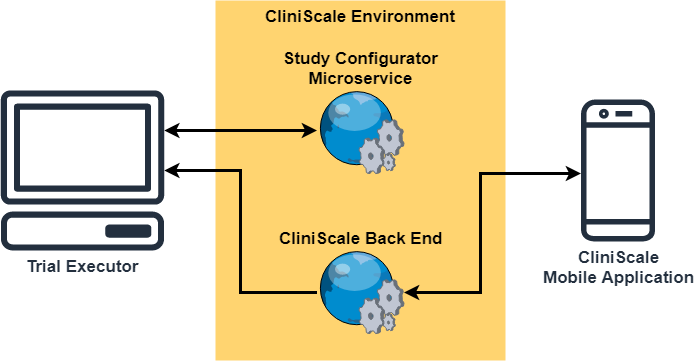
\includegraphics[width=\linewidth]{img/cs-flowchart.png}
  \label{fig:cliniscaleflow}
\end{figure}
\end{frame}

\section{Methodology}
\begin{frame}{Modular Risk Assessment (MoRA)}
\begin{itemize}
    \item Method for security risk assessment developed by Jörn Eichler and Daniel Angermeier at Fraunhofer AISEC in 2015
    \item Flexibility of application in different environments
    \item Customized in order to integrate the MTMT as threat and control catalogue
\end{itemize}
\end{frame}


\begin{frame}{Methodology Overview}
 \begin{figure}[H]
  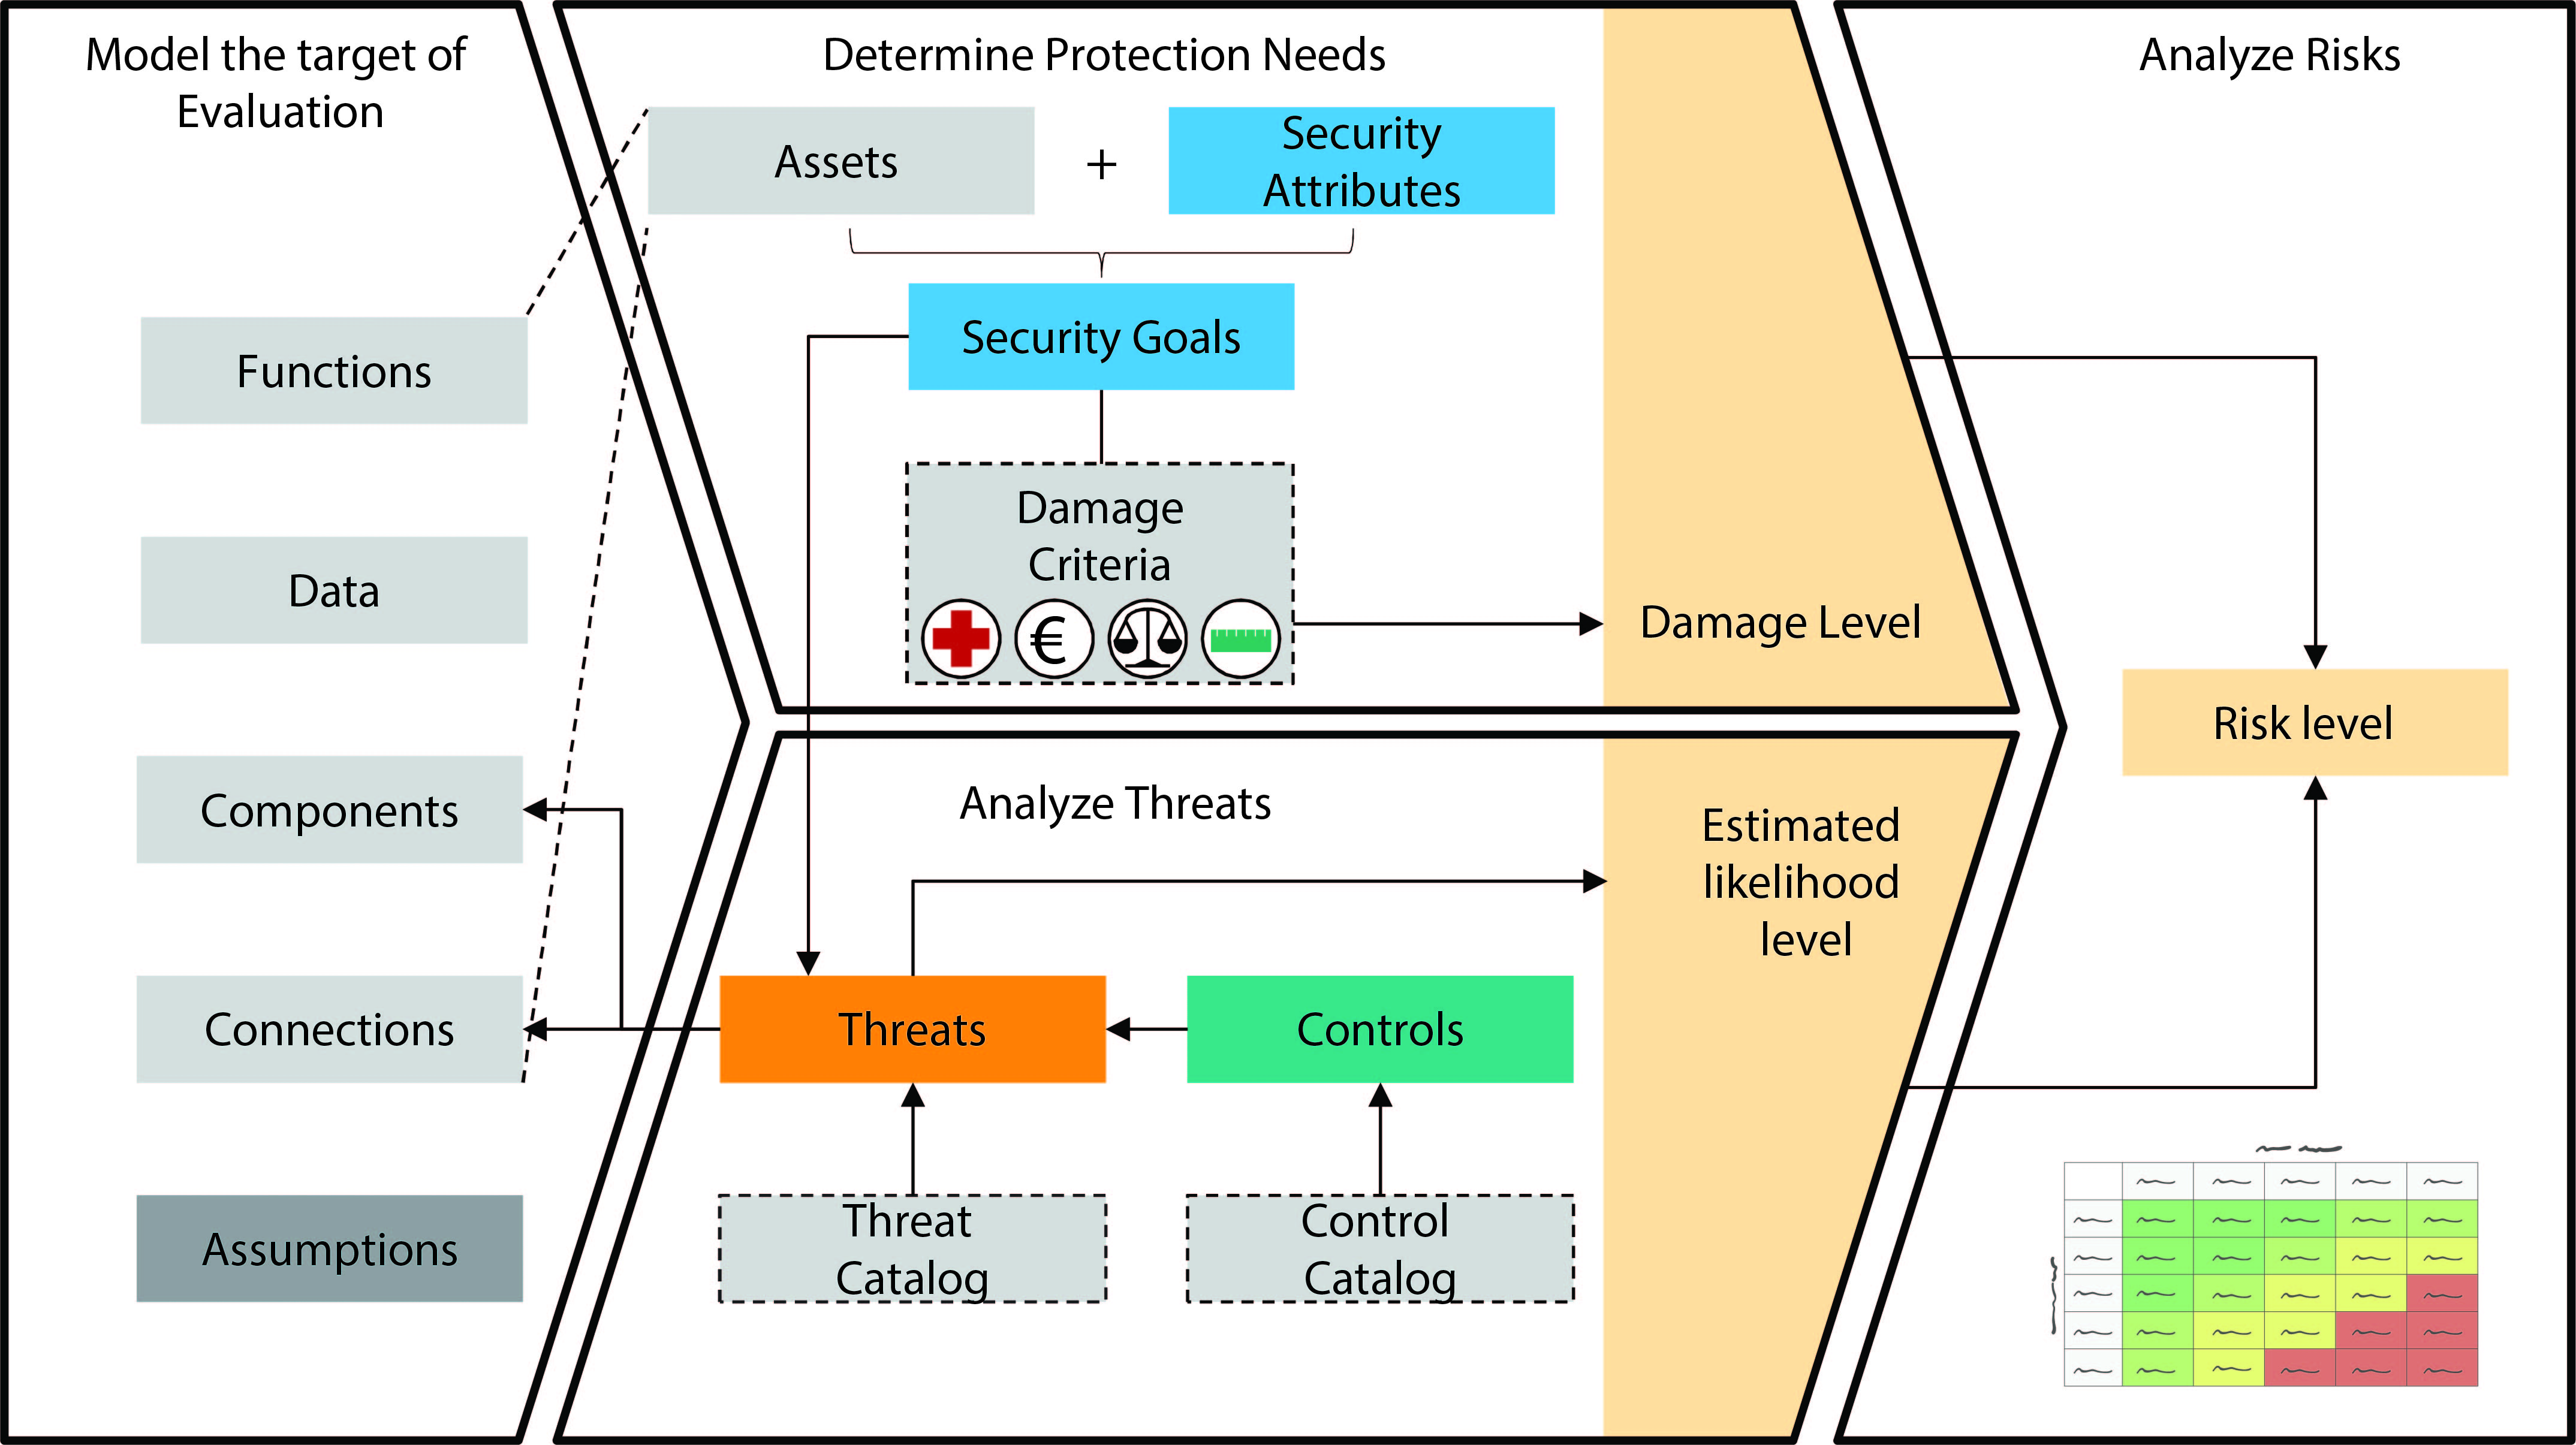
\includegraphics[width=0.9\linewidth]{img/mora-method.jpg}
  \label{fig:mora_overview}
  https://www.aisec.fraunhofer.de/de/presse-und-veranstaltungen/presse/pressemitteilungen/2018/it-sa2018.html
\end{figure}
\end{frame}

\comment{
\begin{frame}{Methodology Overview}
 \begin{figure}[H]
  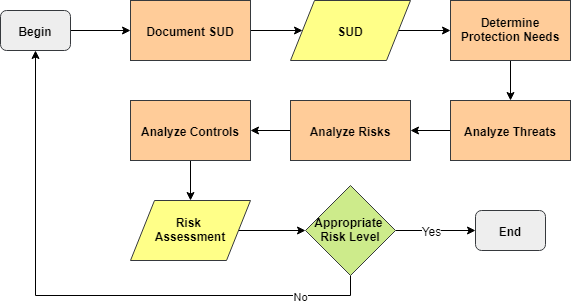
\includegraphics[width=\linewidth]{img/ra_overview.png}
  \label{fig:ra_overview}
  \caption{https://www.aisec.fraunhofer.de/de/presse-und-veranstaltungen/presse/pressemitteilungen/2018/it-sa2018.html}
\end{figure}
\end{frame}
}

\section{Risk Assessment}
\begin{frame}{System Under Development [1/2]}
 \begin{figure}[H]
  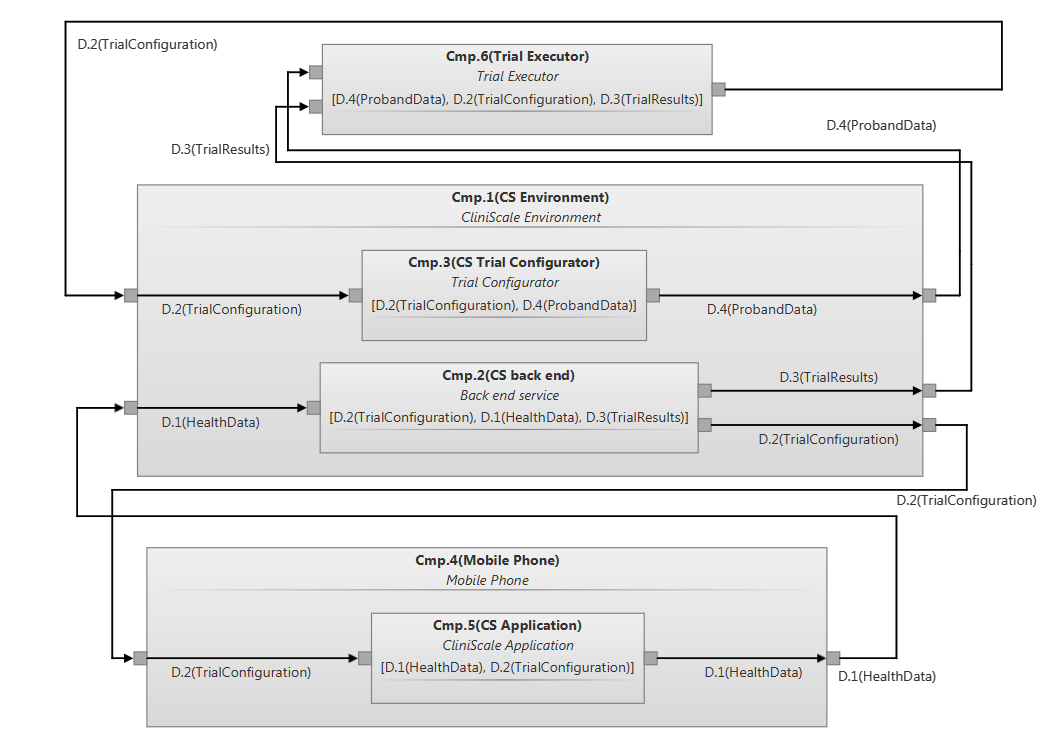
\includegraphics[width=0.9\linewidth]{img/sud_cs.png}
  \label{fig:sud_cs}
 \end{figure}
\end{frame}


\begin{frame}{System Under Development [2/2]}
 \begin{figure}[H]
  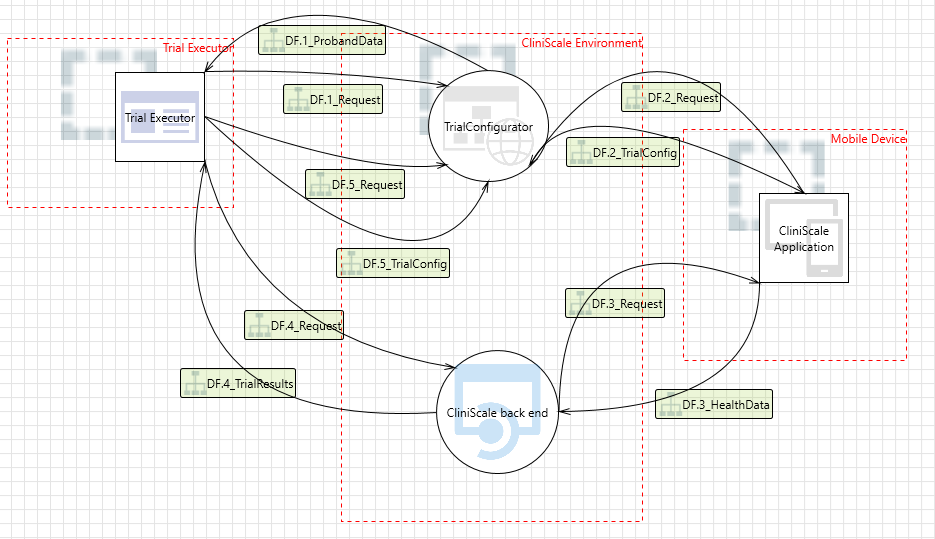
\includegraphics[width=\linewidth]{img/mtmt_model.PNG}
  \label{fig:mtmt_model}
 \end{figure}
\end{frame}


\begin{frame}{Determine Protection Needs [1/2]}
\begin{itemize}
    \item Process of identifying and defining security goals
    \item Assessment Model: Security Goal Classes, Damage Criteria
\end{itemize}
 \begin{figure}[H]
  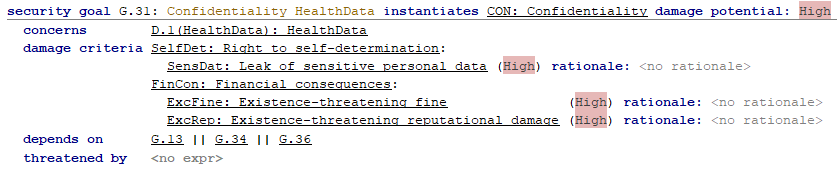
\includegraphics[width=\linewidth]{img/secgoal.png}
  \label{fig:secgoal}
\end{figure}
\end{frame}

%30 Data Flow SG
%24 Data SG
\begin{frame}{Determine Protection Needs [2/2]}
\begin{itemize}
    \item 54 security goals
\end{itemize}
 \begin{figure}[H]
  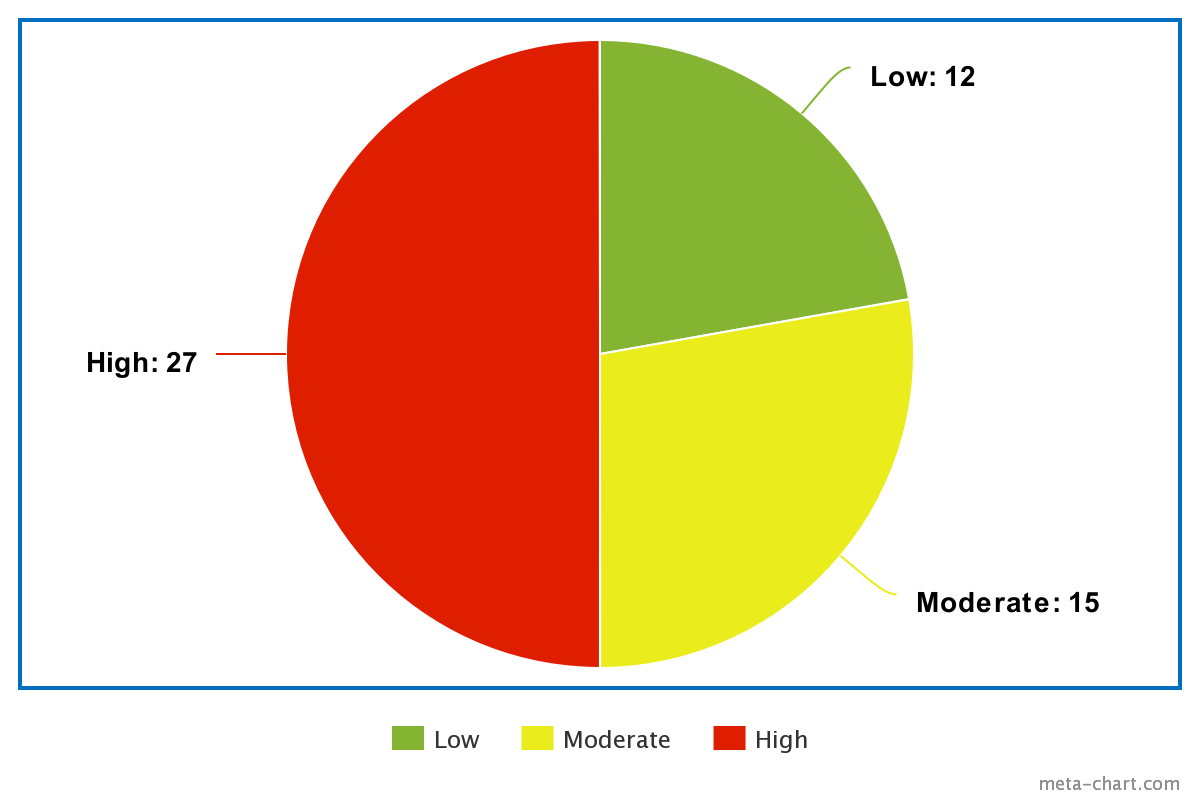
\includegraphics[width=\linewidth]{img/secgoalchart.png}
  \label{fig:secgoalchart}
\end{figure}
\end{frame}


%100 threats from MTMT

\begin{frame}{Analyze Threats [1/2]}
\begin{itemize}
    \item Process of identifying and defining threats
    \item Import threats generated by MTMT
\end{itemize}
 \begin{figure}[H]
  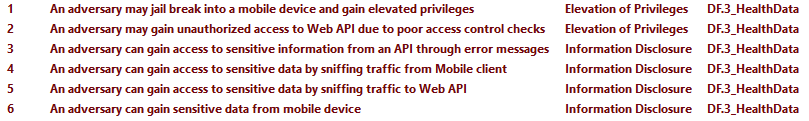
\includegraphics[width=\linewidth]{img/mtmt_threats.png}
  \label{fig:mtmt_threat}
\end{figure}
 \begin{figure}[H]
  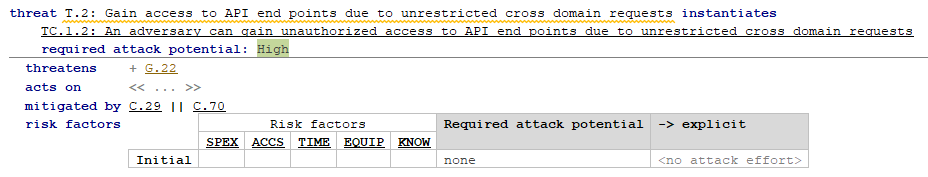
\includegraphics[width=0.9\linewidth]{img/threat.png}
  \label{fig:threat}
\end{figure}
\end{frame}

\begin{frame}{Analyze Threats [2/2]}
\begin{itemize}
    \item 100 threats generated by MTMT
    \item 38 aggregated threats imported
\end{itemize}
 \begin{figure}[H]
  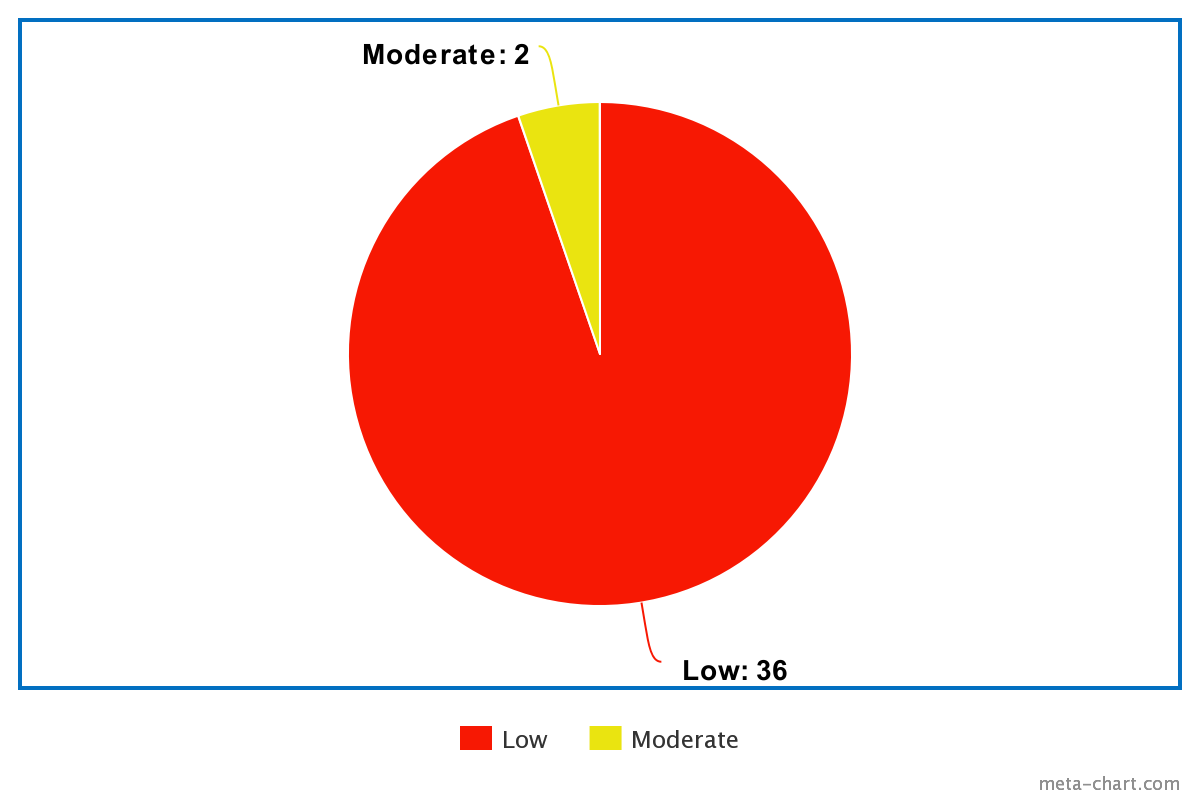
\includegraphics[width=0.9\linewidth]{img/threatchart.png}
  \label{fig:threatchart}
\end{figure}
\end{frame}


\begin{frame}{Analyze Risks}
\begin{itemize}
    \item Process of identifying and defining risk elements
    \item Risk elements provide a summary of the overall risk level
\end{itemize}
 \begin{figure}[H]
  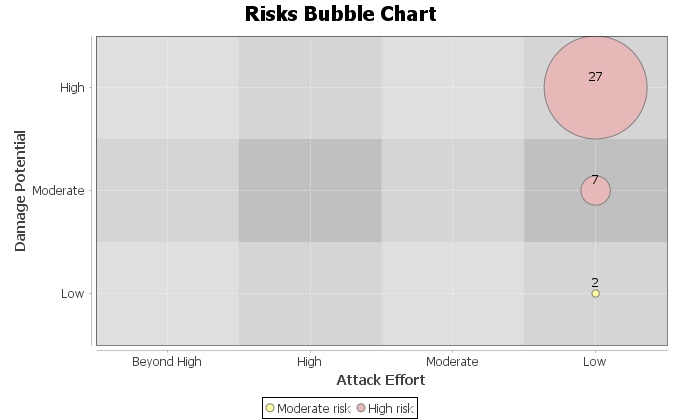
\includegraphics[width=0.8\linewidth]{img/risksBubbleChart.png}
  \label{fig:bubblechart1}
\end{figure}
\end{frame}


\begin{frame}{Establish controls [1/2]}
\begin{itemize}
    \item Process of identifying and defining security control elements
\end{itemize}
 \begin{figure}[H]
  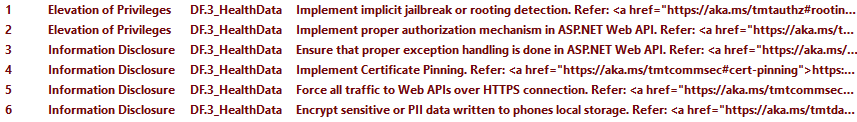
\includegraphics[width=\linewidth]{img/mtmt_controls.PNG}
  \label{fig:mtmtcontrols}
\end{figure}
 \begin{figure}[H]
  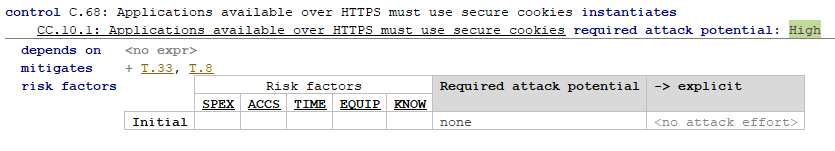
\includegraphics[width=\linewidth]{img/control.PNG}
  \label{fig:control}
\end{figure}
\end{frame}

\begin{frame}{Establish controls [2/2]}
\begin{itemize}
    \item 72 security controls
\end{itemize}
 \begin{figure}[H]
  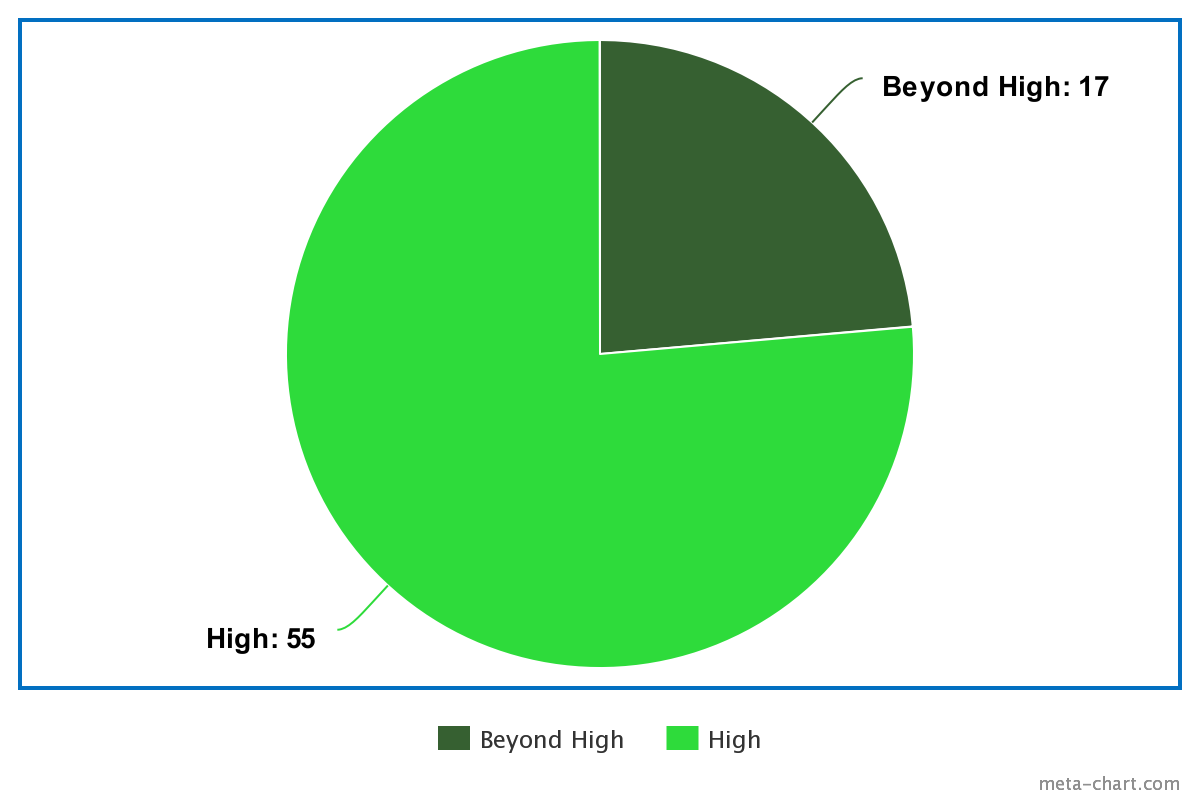
\includegraphics[width=\linewidth]{img/controls.png}
  \label{fig:controlchart}
\end{figure}
\end{frame}


\begin{frame}{Analyze Need for Further Iterations [1/2]}

 \begin{figure}[H]
  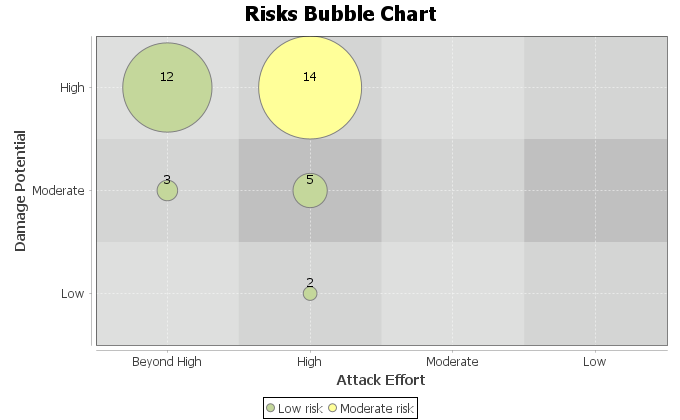
\includegraphics[width=\linewidth]{img/bubble_p2.png}
  \label{fig:bubblechart2}
\end{figure}
\end{frame}

\comment{
\begin{frame}{Analyze Need for Further Iterations [2/2]}
 \begin{figure}[H]
  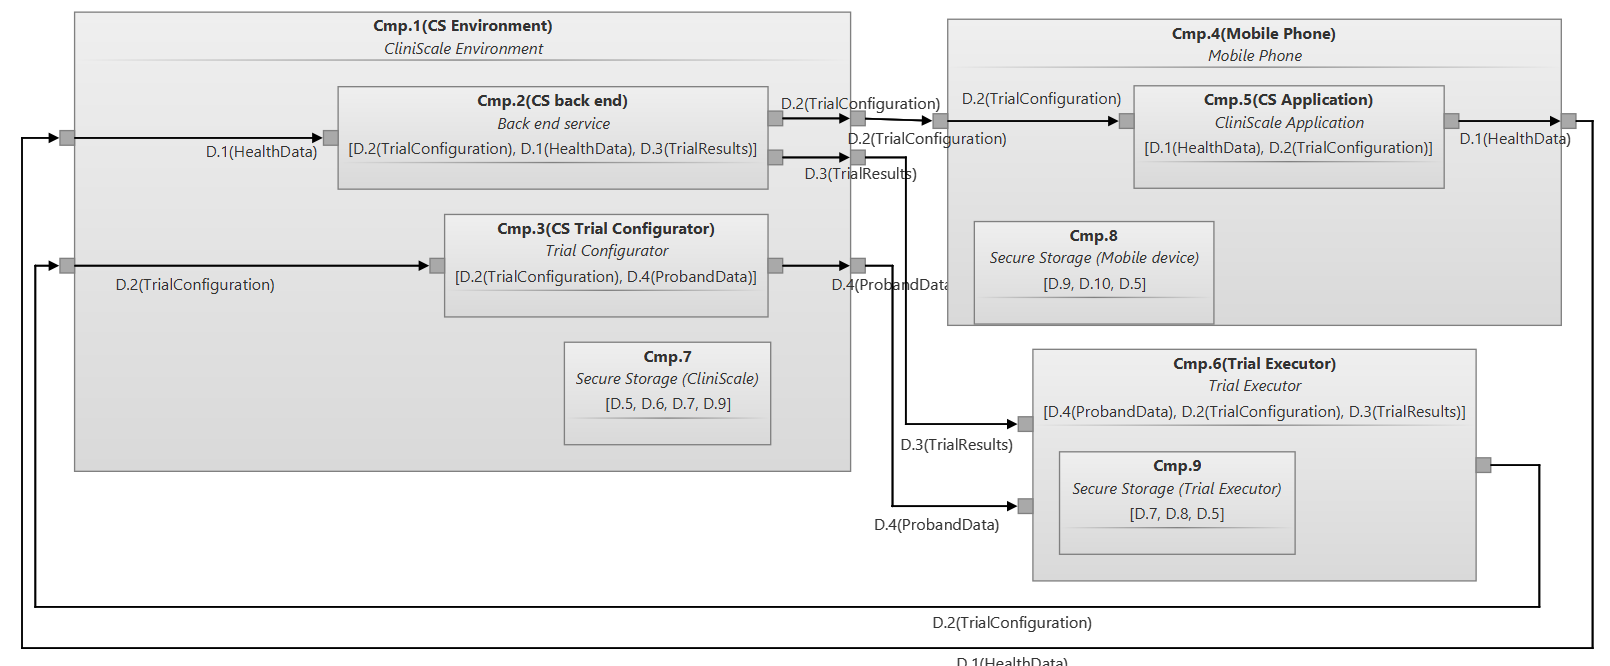
\includegraphics[width=\linewidth]{img/sudp2.png}
  \label{fig:sudp2}
\end{figure}
\end{frame}
}

\section{Implementation Guideline}
\comment{
\begin{frame}{CliniScale System Architecture}
 \begin{figure}[H]
  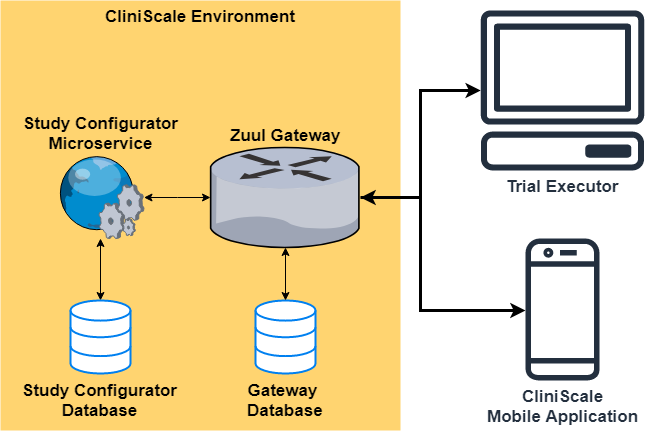
\includegraphics[width=0.8\linewidth]{img/cs-architecture.png}
  \label{fig:cs_architecture}
\end{figure}
\end{frame}
}

\begin{frame}{Technical Implementation Guideline}
\begin{itemize}
    \item Mitigations recommended by the MTMT
    \item Ten categories of mitigations: \textbf{Auditing and Logging}, \textbf{Authentication}, \textbf{Authorization}, \textbf{Communication Security}, \textbf{Configuration Management}, \textbf{Cryptography}, \textbf{Exception Management}, \textbf{Input Validation}, \textbf{Sensitive Data}, \textbf{Session Management}
    \item Recommendations on implementation for every control
    
\end{itemize}
\end{frame}


\begin{frame}{Communication Security}
\begin{itemize}[label={}]
    \item CC.4.4: Force all traffic to Web APIs over HTTPS connection
    \item
\end{itemize}
\begin{itemize}
    \item Hypertext Transfer Protocol Secure
    \item BSI Technical Guidelines \cite{bsitr02}
    \item Implementation supported by the Spring Security Framework
    %\item{\textbf{Article 32: Data Protection by Design and by Default}}  Defines principles the controller has to implement in the process of securing personal data \cite{GDPR32}
\end{itemize}
\end{frame}

\section{Conclusion}
\begin{frame}{Conclusion}
\begin{itemize}
    \item Compliance with the GDPR
    \item Successful integration of the MTMT as threat and control catalogue into the MoRA methodology
    \item Implementation guideline applicable to any client-server infrastructure gathering, storing and processing sensitive personal data
\end{itemize}
\end{frame}


\begin{frame}{Limitations and Future Work}
\paragraph{\textbf{Limitations}}
\begin{itemize}
    \item GDPR investigated for regulations concerning this thesis
    \item Missing information on the required attack potential\\
\end{itemize}
\paragraph{\textbf{Future Work}}
\begin{itemize}
    \item Domain specific threat and control catalogues
    \item Complete security risk assessment of the CliniScale system
\end{itemize}
\end{frame}

\begin{frameWithPicture}{Questions?}{img/questions}
\end{frameWithPicture}% es gibt FUblue, DBbluedark, DBblue

\begin{frame}[allowframebreaks]{References}
\nocite{*}
\printbibliography
\end{frame}

\end{document}